\section{Kapitalstruktur und Kapitalkosten}

\textbf{Kapitalstruktur}: Beschreibt Zusammensetzung der Passivseite, d.h. das Verhältnis von Fremdkapital zu Eigenkapital
\begin{itemize}
	\item Verschuldungsgrad = FK / EK
	\item FK-Quote = FK / (EK + FK)
	\item EK-Quote = EK / (EK + FK)
\end{itemize}

\textbf{Kapitalkosten}: Entsprechen der erwarteten Rendite der Kapitalgeber\\

\textbf{Kapitalstrukturrisiko und Leverage-Effekt}:

Für die Rendite des Eigenkapitals gilt:
$$r_{\scaleto{EK}{4pt}}=\frac{G}{EK}=\frac{r_{\scaleto{GK}{4pt}}\cdot (EK+FK)-(i\cdot FK)}{EK}=r_{\scaleto{GK}{4pt}}+\frac{FK}{EK}(r_{\scaleto{GK}{4pt}}-i)$$

$\rightarrow$ Eigenkapital-Rendite ist eine lineare Funktion des Verschuldungsgrads
\begin{center}
	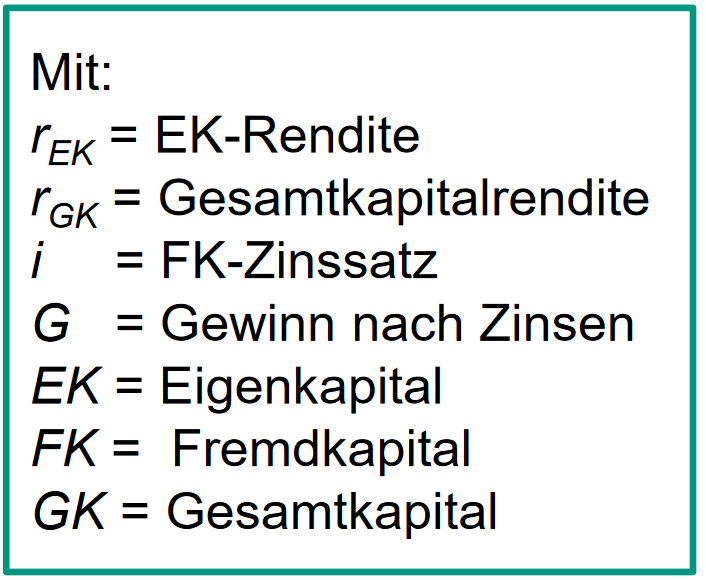
\includegraphics[width=0.25\textwidth]{images/ekr.png}
\end{center}

Risiko des Eigenkapitals:
$$\text{Var}(r_{\scaleto{EK}{4pt}})=(1+\frac{FK}{EK})^2\cdot\text{Var}(r_{\scaleto{GK}{4pt}})$$

Standardabweichung des Eigenkapitals:
$$\text{Std}(r_{\scaleto{EK}{4pt}})=(1+\frac{FK}{EK})\cdot\text{Std}(r_{\scaleto{GK}{4pt}})$$

$\rightarrow$ Stärkere Verschuldung erhöht das EK-Risiko\\

\textbf{Irrelevanz der Kapitalstruktur - Modigliani-Miller-Theoreme}:

\textbf{Annahmen}:
\begin{itemize}
	\item \textbf{Vollkommener und vollständiger} Kapitalmarkt: Keine asymmetrische Information, steuerliche Gleichbehandlung von EK und FK, keine Transaktions-/Insolvenzkosten
	\item \textbf{Rationale Marktteilnehmer}: Keine Arbitrage-Möglichkeit bleibt ungenutzt
	\item \textbf{Gegebenes}, von der Kapitalstruktur unabhängiges \textbf{Investitionsprogramm} des
	Unternehmens
	\item \textbf{Unternehmenswert} ($V$) = Summe der Marktwerte von EK und FK
\end{itemize}
Unternehmen mit dem gleichen Geschäftsrisiko gehören zur gleichen \textbf{Risikoklasse}.

Seien ein verschuldetes (Index $v$) und ein unverschuldetes (Index u) Unternehmen mit den Unternehmenswerten $V_v=EK_v+FK$ und $V_u=EK_u$ gegeben.

\textbf{Behauptung}: Zwei Unternehmen, die sich \underline{nur} hinsichtlich des Finanzierungsrisikos unterscheiden, können auf einem vollkommenen Kapitalmarkt keine verschiedenen Unternehmenswerte haben ($\rightarrow V_v=V_u$)

\textbf{Beweis}: Sei $r$ der risikolose Zinssatz. Sowohl Unternehmen als auch Privatpersonen können sich zu $r$ beliebig verschulden. Betrachte nun folgende zwei Strategien:
\begin{center}
	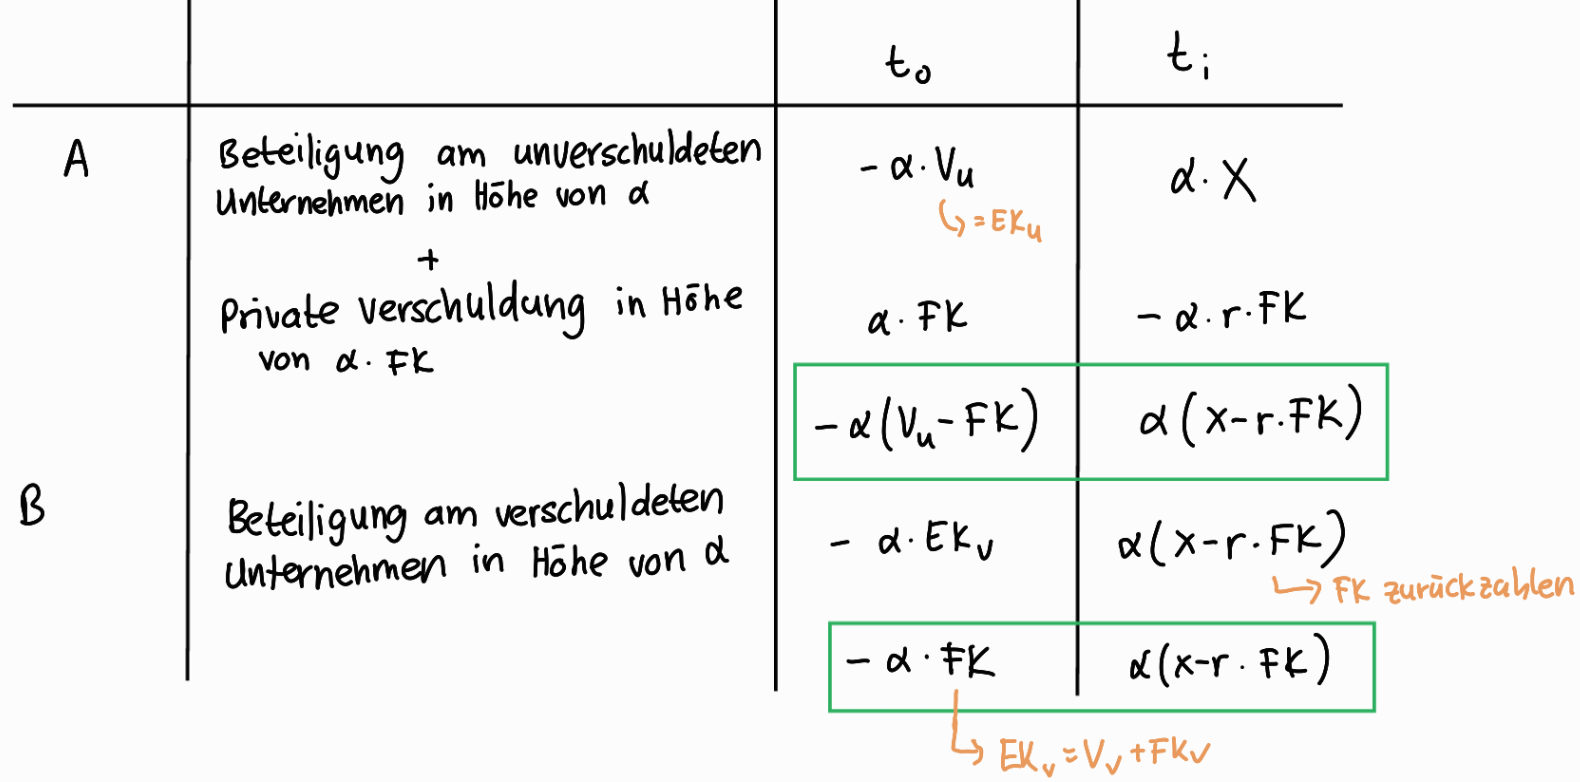
\includegraphics[width=0.8\textwidth]{images/mm.png}
\end{center}
$\rightarrow$ Damit es keine Arbitragemöglichkeit (kostenlos Geld machen) gibt, muss $V_v=V_u$ gelten!

$\rightarrow$ Wenn z.B. $V_u<V_v$, dann leerverkaufe Strategie $B$ und kaufe $A$ $\rightarrow$ Gewinn in Höhe von $\alpha (V_v-V_u)$

\begin{itemize}
	\item \textbf{1. Theorem von Modigliani / Miller}: Die Gesamtwerte zweier Unternehmen der gleichen Risikoklasse, die gleiche erwartete Bruttogewinne aufweisen, sind identisch, und zwar unabhängig von der Kapitalstruktur.
	\item \textbf{2. Theorem von Modigliani / Miller}: Die Eigenkapitalkosten sind eine lineare Funktion des Verhältnisses der Marktwerte von Fremd- und Eigenkapital. Sie sind also eine lineare Funktion des Verschuldungsgrads.
	\item \textbf{3. Theorem von Modigliani / Miller}: Die Gesamtkapitalkosten zweier Unternehmen der gleichen Risikoklasse, die gleiche erwartete Bruttogewinne aufweisen, sind identisch und unabhängig von der Kapitalstruktur. Sie entsprechen den Eigenkapitalkosten eines unverschuldeten Unternehmens.
\end{itemize}

$\rightarrow$ \textbf{Separationstheorem}: Investitionsentscheidungen können unabhängig von Finanzierungsentscheidungen getroffen werden\\

\textbf{Trade-off Theorie und optimale Kapitalstruktur}:

\textbf{Problem}: MM-Modell macht sehr vereinfachende Annahmen, v.a.:
\begin{itemize}
	\item Symmetrische Information
	\item Neutrale Steuern: Debt Tax Shield wird nicht berücksichtigt
	\item Keine Insolvenzkosten
\end{itemize}

\textbf{Gegenläufige Effekte der Verschuldung}:
\begin{itemize}
	\item Höhere Verschuldung führt zu niedrigerer Steuerlast (Debt Tax Shield)
	\item Insolvenzkosten $\rightarrow$ Verschuldung weniger attraktiv, da mit steigender Verschuldung das Insolvenzrisiko steigt
\end{itemize}

\textbf{Berücksichtigung von nicht-neutralen Steuern}:
\begin{itemize}
	\item Für die optimale Kapitalstruktur gilt: Fremdfinanzierung des Unternehmens soviel, dass Steuerlast auf 0 sinkt $\rightarrow V_v>V_u$
\end{itemize}

\textbf{Berücksichtigung von Insolvenzkosten}:
\begin{itemize}
	\item \textbf{Direkte Insolvenzkosten}: Verfahrenskosten
	\item \textbf{Indirekte Insolvenzkosten}: Resultieren daraus, dass Management/ Eigentümer in Krisensituationen sich auf eine Weise zu verhalten, die die Gläubiger schädigt
\end{itemize}

\textbf{Berücksichtigung von Agency-Kosten}: 
\begin{itemize}
	\item \textbf{Agency-Probleme} können den Einfluss der Kapitalstruktur auf das Investitionsprogramm und damit auf Unternehmenswert beeinflussen
\end{itemize}

\textbf{Agency-Probleme}:
\begin{itemize}
	\item Treten auf, wenn:
	\begin{itemize}
		\item bei Trennung von Eigentum und Kontrolle
		\item bei Fremdfinanzierung
		\item \textbf{Beispiele}: Eigentümer - FK-Geber (Investitionsrisiko und Ausfallwahrscheinlichkeit), Eigentümer - Manager
	\end{itemize}
\end{itemize}

\textbf{Anreize eines Managers sind}:
\begin{itemize}
	\item Arbeitseinsatz reduzieren
	\item Konsum am Arbeitsplatz ausweiten (z.B. Privatjet kaufen)
	\item Einzahlungsüberschüsse (\textbf{Free Cash Flow}) investieren und den Wert des Unternehmens damit reduzieren, anstatt diese an die EK-Geber auszuzahlen
\end{itemize}

\textbf{Vorteile des FK}:
\begin{itemize}
	\item Höhere Verschuldung reduziert Marktwert des EK $\rightarrow$ Manager hält einen größeren Anteil des EK des Unternehmens $\rightarrow$ Angleichung der Interessen von Managern und Eigentümern
	\item Höheres Fremdkapital $\rightarrow$ Höhere Auszahlungsverpflichtungen $\rightarrow$ Reduktion des Free Cash Flows
\end{itemize}

\textbf{Nachteile des FK}:
\begin{itemize}
	\item Flexibilitätsverlust durch Covenants und Erhaltung der Liquidität
	\item Asset Substitution: Mehr Anreiz für risikoreichere Entscheidungen, \enquote{da es nicht mein Geld ist}
	\item Debt Overhang: Unterinvestition, da mehr Schulden
	\item Verzögerte Liquidation: Anreiz, Liquidation hinauszuzögern
\end{itemize}

\begin{center}
	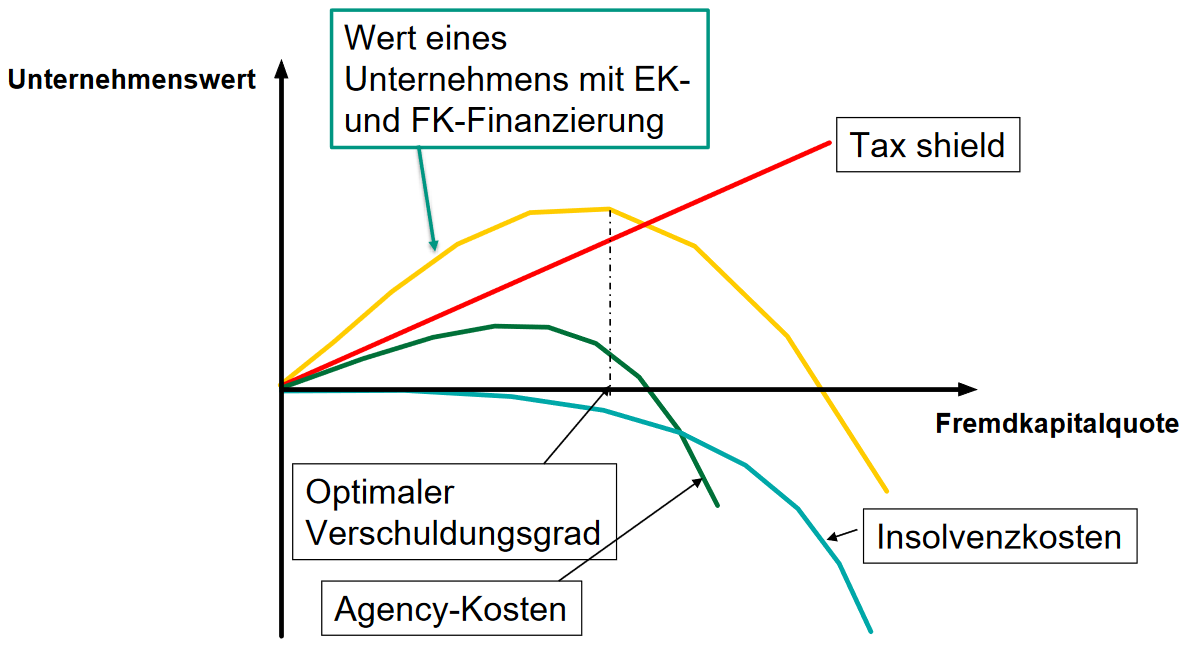
\includegraphics[width=0.55\textwidth]{images/tot.png}
\end{center}

\textbf{Kapitalkosten}:

\textbf{Weighted Average Cost of Capital (WACC)} bei Berücksichtigung von Steuern:
$$WACC=\frac{EK}{EK+FK}\cdot r_{\scaleto{EK}{4pt}}+\frac{FK}{EK+FK}\cdot r_{\scaleto{FK}{4pt}}(1-T)$$
\begin{center}
	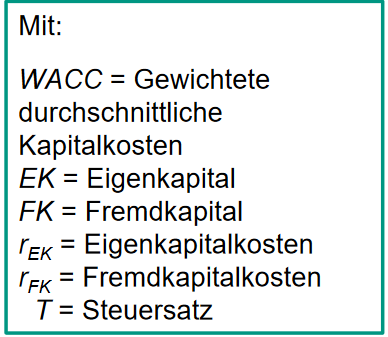
\includegraphics[width=0.25\textwidth]{images/wacc.png}
\end{center}
\begin{itemize}
	\item $r_{\scaleto{EK}{4pt}}$ bzw. $r_{\scaleto{FK}{4pt}}$ = risikofreier Zins + Risikoprämie
	\item WACC dient als Diskontsatz bei der Unternehmensbewertung und bei der Bewertung von Investitionsentscheidungen
	\item Für Gewichte in der WACC-Formel sollten stets Marktwerte verwendet werden ( Marktkapitalisierung für EK und Buchwerte für FK)
	\item Für $r_{\scaleto{FK}{4pt}}$ wird die \textbf{Yield-To-Maturiy} (interner Zinssatz) von Straight Bonds verwendet
	\item $r_{\scaleto{EK}{4pt}}$ wird über das \textbf{CAPM} durch $r_i=r_f+(r_m-r_f)\beta_i$ bestimmt
\end{itemize}
\begin{center}
	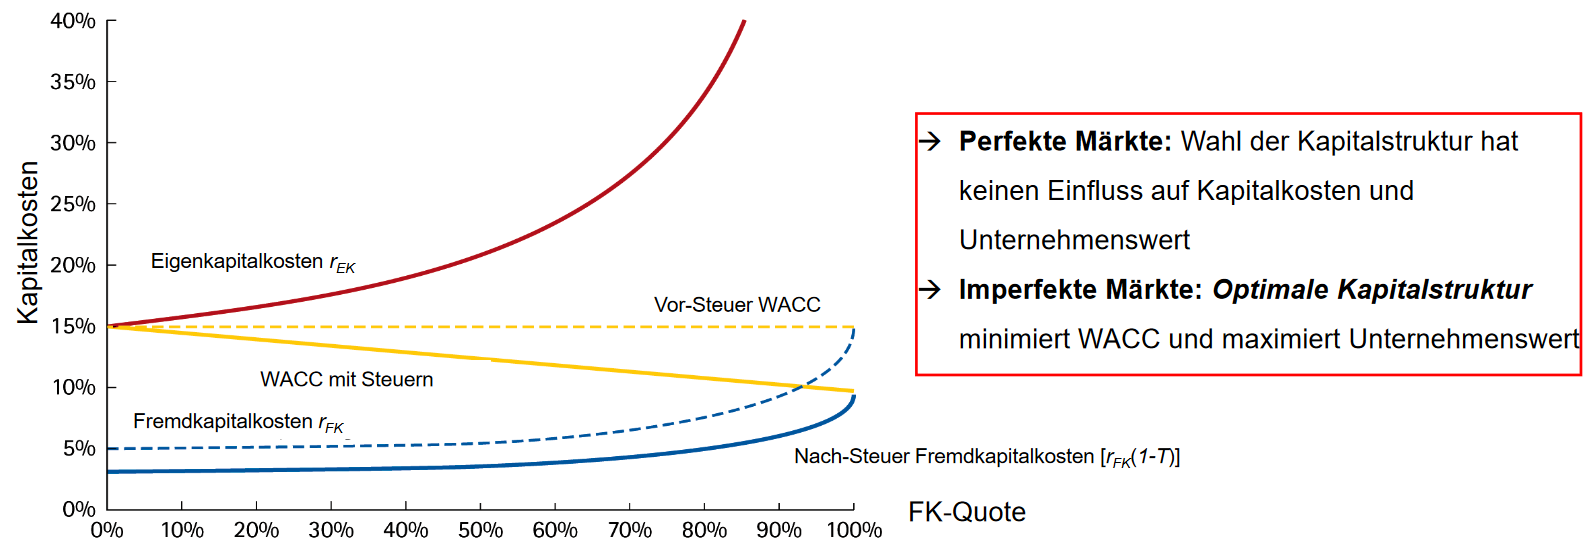
\includegraphics[width=0.9\textwidth]{images/wacc-2.png}
\end{center}